\documentclass[ngerman,twoside,final,web]{../styles/IBB_thesis}
%%%%%%%%%%%%%%%%%%%%%%%%%%%%%%%%%%%%%%%
% OPTIONEN:
% Sprache: ngerman oder english
% Druck:   twoside oder oneside
% Debug:   final   oder draft
% Links:   print   oder web
%
%%%%%%%%%%%%%%%%%%%%%%%%%%%%%%%%%%%%%%%



%%%%%%%%%%%%%%%%%%%%%%%%%%%%%%%%%%%%%%%
% Unterverzeichnisse, in denen Bilder liegen
%%%%%%%%%%%%%%%%%%%%%%%%%%%%%%%%%%%%%%%
\graphicspath{
{01_einleitung/}
{02_beispiel_kapitel/}
}


%%%%%%%%%%%%%%%%%%%%%%%%%%%%%%%%%%%%%%%
% Allgemeine Angaben
%%%%%%%%%%%%%%%%%%%%%%%%%%%%%%%%%%%%%%%



% Name des Bearbeiters
\newcommand{\Autor}{Jonathan Schnitzler}

% Name des Betreuers/der Betreuer
% mehrere Zeilen mit \linebreak
\newcommand{\Betreuer}{Anika Strauß, M.Sc.}

% Titel der Arbeit
\newcommand{\TitelderArbeit}{Künstliche neuronale Netze für statische Berechnung}

% Art der Arbeit:
% Bachelorarbeit, Masterarbeit, Master Thesis
\newcommand{\ArtderArbeit}{Projektarbeit}

% Titelbild (png, jpg, oder gif), Dateiname ohne Endung
% maximal Breite = 15 cm; maximale Höhe = 12 cm
\newcommand{\Titelbild}{titelbild_muster} %TODO

% Studiengang, mit Abschluss in Klammern
\newcommand{\Studiengang}{Simulation Technology (B.Sc.)}

% Monat und Jahr des Anfangs der Bearbeitung
\newcommand{\BearbeitungAnfang}{Oktober 2021}

% Monat und Jahr der Abgabe
\newcommand{\BearbeitungEnde}{Januar 2021}

% Dateiname der Aufgabenstellung als pdf-Datei (ohne .pdf)
\newcommand{\Dateiname}{Aufgabenstellung} %TODO

% Kurzfassung
\newcommand{\textAbstract}{Mithilfe eines künstlichen neuronalen Netzwerks, wird die Verschiebung und Verzerrung eines einfachen Models einer zweidimensionalen Hauswand mit variierender Position von Fenstern und einer Tür unter einer konstanten Querkraft berechnet. Die Daten um das neuronale Netzwerk trainieren, werden dabei von einer finiten Elemente Software erzeugt.}

% Zusätzlicher Abstract in English (optional)
\newcommand{\textAbstractEN}{Using an artificial neural network, the displacement and distortion of a simple model of a two-dimensional house wall with varying position of windows and a door under a constant shear force is calculated. The data to train the neural network are generated by finite element software.} %TODO

% Vorwort (optional)
\newcommand{\textVorwort}{An dieser Stelle kann ein Vorwort bzw.\ eine Danksagung formuliert werden.

Geschweifte Klammern leer lassen, wenn nicht gewünscht.}



\begin{document}

    %%%%%%%%%%%%%%%%%%%%%%%%%%%%%%%%%%%%%%%%%%%%%%%%%
    %
    % VORSPANN:
    % - Titelseiten
    % - Erklärung
    % - Aufgabenstellung
    % - Kurzfassung
    % - Vorwort
    % - Inhaltsverzeichnis
    %
    %%%%%%%%%%%%%%%%%%%%%%%%%%%%%%%%%%%%%%%%%%%%%%%%%
    \vorspann



    %%%%%%%%%%%%%%%%%%%%%%%%%%%%%%%%%%%%%%%%%%%%%%%%%
    %
    % INHALT
    %
    %%%%%%%%%%%%%%%%%%%%%%%%%%%%%%%%%%%%%%%%%%%%%%%%%
    % &latex {


% %%%%%%%%%%%%%%%%%%%%%%%%%%%%%%%%%%%%%%   
% %%%%%%%%%%%%%%%%%%%%%%%%%%%%%%%%%%%%%%
\chapter{Einleitung}
\label{einleitung}


\section{Motivation und Zielsetzung}

Einleitung in das Thema, Motivation

Literaturüberblick: Was gibt es bisher? 

Was ist die Aufgabenstellung, was soll erreicht werden?





\section{Aufbau der Arbeit}
Kurze Beschreibung des Aufbaus der folgenden Arbeit: Wa steht in welchem Kapitel
und wie baut alles aufeinander auf.




    %%%%%%%%%%%%%%%%%%%%%%%%%%%%%%%%%%%%%%%
%
%   G R U N D L A G E N
%
%%%%%%%%%%%%%%%%%%%%%%%%%%%%%%%%%%%%%%%
\chapter{Anwendung der \LaTeX-Vorlage} \label{beispiel_kapitel}
%
%
In diesem Kapitel wird auf Besonderheiten der Vorlage und ihrer Verwendung
eingegangen werden. Es werden Fragen beantwortet, wie Formeln geschrieben
werden, Tabellen gezeichnet werden, Bilder eingefügt werden können\ldots



\section{Optionen dieser Vorlage}

Die Dokumentklasse \verb+IBB_thesis+ unterstützt vier Optionen, für die
es jeweils zwei Möglichkeiten gibt. Es müssen immer alle vier Optionen angegeben werden.
\begin{verbatim}
\documentclass[ngerman,twoside,final,print]{../styles/IBB_thesis}
\end{verbatim}
Die Reihenfolge der Optionen ist beliebig.


\subsection{Deutsch oder Englisch}
Durch die Sprachauswahl Deutsch \verb+ngermen+ oder Englisch \verb+english+
werden die Titelseiten, Überschriften aber auch die Silbentrennung umgeschaltet.


\subsection{Einseitig oder Doppelseitig}
Es gibt die Möglichkeit je nach Ausdruckart (einseitig \verb+oneside+ oder
doppelseitig \verb+twoside+) die Vorlage umzustellen. Dies ist wichtig, das
sonst bei einem einseitigem Druck einige weiße Seiten mit Seitenzahl gedruckt würden,
die bei doppelseitigen Druck richtigerweise auf der Rückseite landen würden.


\subsection{Entwurf oder Druckversion}
Mit der Option \verb+draft+ kann einerseits der Übersetzungsvorgang beschleunigt
werden (Bilder werden z.B. nur als Umrandung angezeigt), andererseits werden
Label im pdf-Dokument angezeigt, so dass Verweise auf Bilder und Formeln
einfacher gesetzt werden können. Für den Druck muss diese Option unbedingt auf
\verb+final+ gesetzt werden.


\subsection{Print oder Web}
Mit der Option \verb+web+ werden Verweise innerhalb des Dokuments als Links
erzeugt, d.h. man kann z.B. vom Inhaltsverzeichnis zu den einzelnen Abschnitten
springen oder von einem Verweis zum passenden Bild, Tabelle, Formel.

Für den Ausdruck muss diese Option unbedingt auf \verb+print+ gesetzt werden,
für die elektronische Version sollte sie auf \verb+web+ gesetzt werden.



\section{Allgemeine Angaben}

Relativ weit oben in thesis.tex können allgemeine Angaben gemacht werden die
immer wieder benötigt werden und automatisch auf dem Deckblatt etc. übernommen
werden


\section{Neues Kapitel anlegen}

Für jedes Kapitel sollte ein neues Verzeichnis/Ordner angelegt werden. In diesem
Verzeichnis sollte/n die .tex-Datei, die Grafiken und die Diagramme gespeichert
werden.
Anschließend muss in der Hauptdatei thesis.tex mit dem Befehl
\verb+\input+ die neue .tex-Datei eingebunden werden.
Damit Bilder in dem neuen Verzeichnis gefunden werden, muss dieses dem
\verb+\graphicspath+ hinzugefügt werden (siehe Abschnitt~\ref{sec:Bilder}).


\section{Formeln}
Zum besseren Verständnis der folgenden Ausführungen sollte das pdf und der
Quelltext "`04\_beispiel\_kapitel.tex"' gleichzeitig betrachtet werden.

Eine Formel wird immer als Quelltext angegeben. Möchte man beispielsweise ein
$\al$ schreiben muss \verb+\alpha+ angeben werden. Eine besonders
hilfreiche Internetseite hierzu ist
\url{http://de.wikipedia.org/wiki/Hilfe:TeX}.
Hier kann fast jeder griechischer Buchstabe oder mathematisches Formelzeichen
gefunden werden. Wer Formeln kompakter und übersichtlicher gestalten möchte,
sollte die vom IBB definierten Kurzbezeichnungen für griechische Buchstaben,
Formelzeichen, Einheiten\ldots verwenden. Eine Zusammenfassung aller vordefinierter Befehle findet sich in
einem separaten PDF names "`Abkuerzungen.pdf"' .
Durch die Verwendung dieser Abkürzungen (beispielsweise \verb+\al+ statt
\verb+\alpha+) können Formatierungsfehler automatisch vermieden werden.

\subsection{Äußere Form}

Soll eine kurze Formel, wie $\si = \frac{F}{A}$, im Satz eingebetet werden,
muss diese in \verb+$+-Zeichen eingeschlossen werden. Freistehende Formeln
werden in der extra Umgebung \verb+align+ definiert:
%
\begin{align}
\Bx = \Bph (\BX,t).
\end{align}
%
Soll der Folgetext direkt an die Formel ohne Absatz angrenzen, ist darauf zu
achten keine Leerzeilen zwischen Formel (\verb+align+-Umgebung) und Vor- und
Nachlauftext einzufügen. Um den Quellcode trotzdem übersichtlich zu gestalten,
können \verb+%+-Zeichen eingefügt werden, die zum Auskommentieren der Zeile
führen.

Werden zwei oder mehr Zeilen in einer \verb+align+-Umgebung benötigt, wird mit
dem Befehl \verb+\\+ die Zeile umgebrochen und mit einem
\verb+&+-Zeichen die Formeln zueinander ausgerichtet, beispeilsweise hier am
ersten Gleichheitszeichen:
%
\begin{align}
\dot\Bu(\BX, t) &= \fracpt{\Bph(\Bx, t)}{t}= \fracpt{\Bu(\Bx, t)}{t} ,
\\
\ddot\Bu(\BX, t) &= \fracpt{\dot\Bu(\Bx, t)}{t} .
\end{align}
%
Sollen mehere Formeln nebeneinander angeordnet werden, können mehrere
\verb+&+-Zeichen verteilt werden, um die gewünschte Anordnung zu erhalten.
%
\begin{align}
a_{11}& =b_{11}&
a_{12}& =b_{12}&
a_{13}& =b_{13}&\\
a_{21}& =b_{21}&
a_{22}& =b_{22}+c_{22}&
a_{23}& =b_{23}
\end{align}
%
Eine spezielle Anordnung wie
\begin{align}
\Bt_\RT =
\begin{cases}
  \Bt_\RT^\text{test},  & \text{wenn } \PH(\Bt_\RT^\text{test}) \leq 0\\
  - \mu_\RT \la_\RN \frac{\Bt_\RT}{\| \Bt_\RT \|}, & \text{sonst}
\end{cases}
\end{align}
kann auch Sinn machen, wenn eine Variable, hier $\Bt_\RT$, für zwei oder mehr Fälle
eine andere Definition aufweist.

Werden mehrere Formeln in einer \verb+align+-Umgebung zusammengefasst, erhält
jede Zeile eine eigene Gleichungssnummer. In manchen Fällen ist es aber ratsam,
nur eine Gleichungssnummer zu haben. Dafür muss eine \verb+split+-Umgebung
innerhalb der \verb+align+-Umgebung definiert werden:
%
\begin{align}
\begin{split}
\de W_{\textnormal{PvV}}^\RF =
&\underbrace{\int_{\OM_0} \de\Bu \cdot [ \rho_0 \ddot\Bx ] \dO_0
}_{\de W_\textnormal{PvV}^{\textnormal{kin}}} +
\underbrace{\int_{\OM_0} \de\BE : \BS \dO_0}_{\de W_\textnormal{PvV}^{
\Rint}}  \\
&\underbrace{- \int_{\OM_0} \de\Bu \cdot [\rho_0 \Bb] \dO_0
-\int_{\GA_\RN} \de\Bu \cdot \hat\Bt_0
\dif\GA_\RN}_{-\de W_\textnormal{PvV}^{\Rext}}
= 0 .
\end{split}
\label{eq:PvV}
\end{align}
%
Allerdings kann eine Formel in der \verb+split+-Umgebung nur noch an einem
\verb+&+ Zeichen ausgerichtet werden. Soll noch eine weitere Information
hinzukommen, kann mit dem Abstandshalter \verb+\quad+ gearbeitet werden:
\begin{align}
\begin{split}
\la \in \CM^{-} \quad \quad \CM^{-} &= \Bigl\{ \la : \GA_\RC \to
\BBR^{-} \mid \la \in \BQ' (\GA_\RC), \la \leq 0 \Bigr\} , \\
\de\la \in \CM^{+} \quad \quad \CM^{+} &= \Bigl\{ \de\la : \GA_\RC \to
\BBR^{+} \mid \de\la \in \BQ'(\GA_\RC), \de\la \geq 0 \Bigr\} .
\end{split}
\label{eq:lag_multi}
\end{align}
Möchte man im Nachhinein auf die Formel
referenzieren, ist ihr ein \verb+\label{Name}+ zuzuordnen. Nun kann mit \verb+\eqref{Name}+ auf die
Formel~\eqref{eq:PvV} oder die Formel~\eqref{eq:lag_multi} verwiesen werden. Um
automatisch gesetzte Umbrüche zwischen dem Wort "`Formel"' und der
Gleichungsnummer zu unterbinden, ist ein geschütztes Leerzeichen \verb+~+ zu
verwenden. Dies ist auch beim Verweis auf Bilder sehr sinnvoll.

Des Weiteren gilt:
\begin{itemize}
  \item Formeln sollten in einen Satz eingebaut werden und somit auch mit einem
  Satzzeichen wie Komma oder Punkt versehen werden.
  \item Jede Variable der Formeln sollte mindestens einmal erklärt werden.
  Variable und ihr Name sollten eindeutig zuordenbar sein.
  \item Es sollte keine \verb+eqnarray+ oder \verb+array+-Umgebung
  genutzt werden, da falsche Abstände zwischen Formelzeichen entstehen.
\end{itemize}

\subsection{Formelinhalt}

Für die Schreibweise von Formeln gibt es ebenfalls einige Regeln. Die
wichtigsten sind im Folgenden zusammengefasst. Für vertiefende Studien lohnt es
sich die Online-Dokumentationen "`amsmath"' und "`mathtools"' anzuschauen.

\subsubsection{Skalare, Vektoren, Matrizen}

Bezeichnungen für Skalare werden im Allgemeinen kursiv geschrieben $y=mx+c$.
Selbes gilt für Bezeichnungen wie $x$-Achse, $x$-Richtung oder $\hat{u}_x$.
%
Vektoren und Matrizen hingegen werden "`fett"' und gerade
geschrieben, wie beispielsweise der Normalenvektor $\Bn$ oder die
Steifigkeitsmatrix $\BK$. Auch hier ist die Verwendung der Kurzschreibweisen
hilfreich, denn $\Bn$ lässt sich kurz mit \verb+\Bn+ statt lang mit
\verb+\mathbf{n}+ erzeugen. Hierbei steht der Buchstabe "`B"' für "`bold"'. Wird
ein Vektor definiert, beispielsweise durch
\begin{align}
\de\Bd = \begin{bmatrix}
 \de\Bd_1 \\
 \de\Bd_2 \\
 \vdots \\
 \de\Bd_{n}
\end{bmatrix}
\end{align}
ist eine \verb+bmatrix+-Umgebung zu verwenden. In speziellen Fällen, bei denen
eine nicht zentrierte Ausrichtung der Einträge sinnvoll ist, kann eine
\verb+bmatrix*+-Umgebung genutzt werden:
\begin{align}
\BF &= \begin{bmatrix*}[r]
 1 \\
 -1\\
 1 \\
 -1
\end{bmatrix*}
&& \text{ist besser als} &
\BF &= \begin{bmatrix}
 1 \\
 -1\\
 1 \\
 -1
\end{bmatrix}
&& \text{oder} &
\BF &= \begin{bmatrix*}[l]
 1 \\
 -1\\
 1 \\
 -1
\end{bmatrix*} .
\end{align}


\subsubsection{Indizes}

Prinzipiell werden zwei unterschiedliche Arten von Indizes unterschieden:
kursive und nicht kursive. Kursive Indizies müssen verwendet werden, wenn
der Buchstabe eine Variable beschreibt, wie beispielsweise in einer Summation
über $I$:
\begin{align}
\Bu \approx \Bu^h (\Bxi) = \sum_{I=1}^n N_I(\Bxi) \Bd_I
\label{eq:verschiebungsansatz}
\end{align}
oder in der Update-Vorschrift der Beschleunigung
\begin{align}
\ddot\Bu^{i+1} = \ddot\Bu^{i}+\DE \ddot\Bu .
\label{eq:update_iteration}
\end{align}
Wenn nun im nachfolgenden Satz auf
den kursiven Index $I$ bzw. $i$ hingewiesen werden
soll, muss $I$, bzw. $i$ auch hier kursiv und nicht gerade geschrieben
werden.

Nicht kursiv sind Indizes, die für eine Bezeichnung stehen wie der Index
$(\bullet)_\RN$ für Normalenrichtung. Statt \verb+$\textnormal{N}$+ kann hier
die Kurzschreibweise \verb+$\RN$+ verwendet werden. Der Buchstabe "`R"' geht auf
das Wort "`Roman"' zurück.
In der folgenden Formel sind beispielsweise die Bezeichnungen "`F"' für Festkörper, "`kin"' für kinetisch, "`int"' für
intern oder "`ext"' für extern gerade zu schreiben.
\begin{align}
\begin{split}
\de W_\RF^h (\Ba, \Bd) &= \de W_{\textnormal{kin}}^h+ \de W_{\Rint}^h-
\de W_{\Rext}^h  \\
&= \de \Bd^\RT \Bf_\textnormal{kin}(\Ba)
+ \de \Bd^\RT \Bf_\Rint(\Bd)
- \de \Bd^\RT \Bf_\Rext = 0
\end{split}
\label{eq:semi_dis_virt_arbeit}
\end{align}
%
Über den Diskretisierungsindex $(\bullet)^h$ kann man sich an dieser Stelle
streiten, da er für den Diskretisierungsansatz und damit für eine Bezeichnung
steht und so gerade geschrieben werden könnte. Historisch wurde der Buchstabe
$h$ aber für die Seitengröße eines Elements eingeführt und verweist damit auf eine skalare Variable, die kursiv
geschrieben wird. Hier im Institut wird deshalb die Auffassung vertreten den
Verweis auf die Diskretisierung $(\bullet)^h$ kursiv zu schreiben.



\subsubsection{Operatoren}

Rechenoperatoren wie der natürliche Logaritmus "`$\ln$"', der Sinus "`$\sin$"' oder auch
"`$\operatorname{arg\,min}$"', "`$\grad$"' dürfen nie kursiv geschrieben werden,
da sie für eine spezielle Rechenoperation stehen. Hier reicht es allerdings
nicht aus diese mit einem \verb+$\textnormal{}$+-Befehl gerade zu rücken,
sondern falls noch nicht vordefiniert, muss eine spezielle
\verb+\operatorname{}+-Umgebung genutzt werden, wie in
\begin{align}
\bar\Bx (\Bx^\Rs) = \underset{\Bx^\Rm \in \ga_\RC^\Rm
}{\operatorname{arg\,min}} \| \Bx^\Rs - \Bx^\Rm(\Bxi) \|
\end{align}
zu sehen. Für viele Rechenoperationen gibt es schon vordefinierte Befehle wie
\verb+\Div+ für $\Div$ oder \verb+\Grad+ für $\Grad$ oder \verb+\dx+ für $\dx$.
Zu finden sind diese in der Datei "`Abkuerzungen.pdf"' in Kapitel~0.4.
Da die Transponierte ebenfalls einen Operator darstellt, gilt hier auch die
Regel des Gerade-Schreibens. Allerdings reicht die Schreibweise
\verb+\RT+ für den Index $\RT$ völlig aus.

Das Symbol des Skalarprodukts "`$\cdot$"' wird in vielen Arbeiten zu häufig
genutzt. Werden skalarwertige Variablen mit einander multipliziert wird
üblicherweise kein Produktzeichen "`$\cdot$"' zwischen den Faktoren angeben,
siehe $y=mx+c$.
Das Symbol "`$\cdot$"' steht vielmehr für das Skalarprodukt von Vektoren
z.\,B. $\|\Bx\| = \sqrt{\Bx \cdot \Bx}$ oder allgemein für die einfache
Verjüngung, das Symbol "`$:$"' für die doppelte Verjüngung.


\subsubsection{Einheiten}

Einheiten sollten in Rechenbeispielen mit angegeben werden. Sie sind nicht
kursiv zu schreiben und weisen zur Zahl einen halben Abstand (\verb+\,+) auf,
z.\,B. $E= 100\UkNpmq$ oder $t=0,1\Um$. An dieser Stelle lohnt es sich von den
vordefinierten Einheitenbefehlen Gebrauch zu machen, da diese sowohl den halben
Abstand als auch die richtige Schriftneigung aufweisen.

Wenn Achsenbeschriftungen von Diagramme mit einer Einheit versehen werden
sollen, gibt es zwei Varianten dies zu tun:  $u_y$ in m oder $u_y$ / m .




\section{Tabelle erzeugen}

Tabellen werden in einer \verb+table+-Umgebung mit eingebetteter
\verb+tabular+-Umgebung definiert. Die \verb+tabular+-Umgebung erlaubt eine
einfache Ausrichtung der einzelnen Spalten mit den Befehlen \verb+c+ für
mittig, \verb+l+ für linksbündig, \verb+r+ für rechtsbündig und  \verb+S+ für
eine Ausrichtung am Dezimaltrennzeichen.

\begin{table}[t]
\centering
\begin{tabular}[H]{@{}cccSS@{}}
  \toprule
  \scriptsize{Netz} & \scriptsize{Elementanzahl} &
  \scriptsize{Netzgröße $h$ in cm} &
  \scriptsize{Verzerrungsenergie in J}  &
  \scriptsize{Error [\%] Greville}\\
  \midrule
  1 & 1     & 12,5664  & 1,15122 & 23,1623\\
  2 & 4     & 6,28319  & 1,36973 & 8,57804\\
  3 & 16    & 3,14159  & 1,67895 & 12,0610\\
  4 & 64    & 1,57080  & 1,48293 & 1,02218\\
  5 & 256   & 0,78540  & 1,50929 & 0,73691\\
  6 & 1024  & 0,39270  & 1,49694 & 0,08755\\
  7 & 4096  & 0,19635  & 1,49839 & 0,00957\\
  8 & 16384 & 0,09817  & 1,49825 &  0,12 \\ \bottomrule
\end{tabular}
\caption{Anzahl an Elementen, Netzgröße, Verzerrungsenergie und relativer
Fehler.}
\label{tab:strain_energy}
\end{table}

Tabellen, wie Tabelle~\ref{tab:strain_energy}, sollten im Text beschrieben
und es sollte auf sie referenziert werden.



\section{Einbinden von Bildern}
\label{sec:Bilder}

Die Bilder sollten in dem Ordner des jeweiligen Kapitels gespeichert sein.
Jeder Ordner in dem Bilder liegen, muss zunächst in der Hauptdatei thesis.tex
angegeben werden. Dies geschieht durch den Befehl \verb+\graphicspath+.
Der Pfad muss relativ zur Hauptdatei, d.h. thesis.tex, angegeben werden und
mit einem "`\verb+/+"' beendet werden.

\begin{enumerate}
  \item figu tippen und Strg + Leertaste drücken
  \item Im Dialogfenster figure - Template for figure wählen. Es erscheint
  folgender Text:
\begin{verbatim}
  \begin{figure}[t]
    \begin{center}\small

    % Grafik: png, jpg, pdf
    \includegraphics[width=1.0\textwidth]{filename}
    % Inkscape Build
    \includesvg{filename}
    % Gnuplot mit tkiz
    \includegp{filename}

    \caption{figureCaption}
    \label{fig:figureLabel}
  \end{center}
\end{figure}
  \end{verbatim}
  \item Für png, jpg, PDF Dateien den ersten include-Befehl behalten und die
  beiden anderen löschen.
  Für Inkscape svg Dateien oder Gnuplot gp Dateien entsprechend vorgehen.
  Der \textit{filename} ist dabei der Pfad zum dem Bild, bzw. dem gnuplot
  relativ zur Hauptdatei, d.h. thesis.tex, gesehen
\end{enumerate}
An dieser Stelle hier wird nun das Inkscape-Bild Abbildung~\ref{fig:poly} eingebunden.
%%
%% Inkscpae Bild mit automatischem Übersetzen
\begin{figure}[t]
  \centering\small
    \includesvg{02_beispiel_kapitel/inkscape_01}
  \caption{Inkscape Bild.}
  \label{fig:poly}
\end{figure}
Sollen Bilder, wie in Abbildung~\ref{fig:drei_bilder} zu sehen, nebeneinander
angeordnet werden, da es z.B.
Ausschnitte eines Videos sind, muss für jedes Bild eine Minipage angelegt werden.
\begin{figure}[b]
\begin{minipage}[t]{4cm}
\centering
    \includesvg{02_beispiel_kapitel/Kreis_1}
    \scriptsize{Lastschritt 1}
\end{minipage}
\hfill
\begin{minipage}[t]{4cm}
\centering
    \includesvg{02_beispiel_kapitel/Kreis_2}
    \scriptsize{Lastschritt 4}
\end{minipage}
\hfill
\begin{minipage}[t]{4cm}
\centering
    \includesvg{02_beispiel_kapitel/Kreis_3}
    \scriptsize{Lastschritt 8}
\end{minipage}
\caption{Drei Bilder nebeneinander.}
\label{fig:drei_bilder}
\end{figure}
Gleiches gilt wenn beispielsweise eine Formel neben einen Bild gezeigt werden
soll, siehe Abbildung~\ref{fig:Bild_mit_Formel}:
\begin{figure}[t]
\begin{minipage}{10cm}
\centering
    \includesvg{02_beispiel_kapitel/Tragwerk}
\end{minipage}
\begin{minipage}{4cm}
\begin{align*}
E &= 100 \UkNmq \\
F &= 1 \UkN
\end{align*}
\end{minipage}
\caption{Ein Bild mit Formel daneben.}
\label{fig:Bild_mit_Formel}
\end{figure}

Wichtig: Bilder werden immer in der Originalgröße eingefügt. Ist ein Bild zu
groß, so muss es in Inkscape selber kleiner skaliert werden. Nachträglich
Skalierungsänderungen in \LaTeX-Dokument würden auch die Schrift im Bild kleiner
skalieren, was unerwünscht ist.

Auf gezeigte Graphiken sollte immer im Text verwiesen werden und diese auch
ausführlich beschrieben und diskutiert werden.


\section{Gnuplot}
Im Folgenden werden anhand der Vorlage "`Beispielplot.gp"' die grundlegenden
Funktionen von Gnuplot dargestellt. Wie z.B. die Festlegung der Größe des
Zeichenbereichs, die Achsenbeschriftung, welche Kurven geplottet werden, etc.

Während des Übersetzungsvorgangs wird aus der Datei "`Beispielplot.gp"'
automatisch eine Datei "`Beispielplot.tex"' erstellt. Diese übersetzten Befehle
können nun vom pdflatex verarbeitet werden.

\subsection{Erläuterungen zur Beispieldatei "`Beispielplot.gp"'}
In der Hauptdatei "`Beispielplot.gp"' sind die wichtigsten Stellen bereits
kommentiert. Die Struktur und die wichtigsten Befehle können erkannt werden.

\begin{verbatim}
# Groesse des Zeichenbereichs festlegen
set terminal tikz color size 10cm, 7cm
set output '02_beispiel_kapitel/Beispielplot.tex'

#set termoption dash

# Achsentyp definieren mit Netz in Zeichenflaeche
set grid
set xzeroaxis lt -1 linewidth 1
set yzeroaxis lt -1 linewidth 1

# x-/y-Achse festelegen
set xrange [0:15.708]
set yrange [-3.2:0.4]

# Unterteilung der Achsen
set xtics 2
set ytics 0.4

# Achsenbeschriftung
set xlabel 'Pfad'
set ylabel ' $M_{xx}$'

# Lage und Groesse der Legendenbox
set pointsize 2.0
set key box
set key bottom right

# Beschriftung im Zeichenbereich setzen
set label "Spitze" at 1.7,-1.8

# Definieren einer kontinuierlichen Referenzloesung
Konstante=1.0
Ref(x)=-cos(x/10.0)*Konstante*Konstante*Konstante

# Zeichnen der Kurven
plot\
'02_beispiel_kapitel/Datenreihe1.data' u 1:2  title 'Daten 1'...
      with points  pt 4  ps 2 linecolor rgb "red" ,\
'02_beispiel_kapitel/Datenreihe2.data' u 1:2  title 'Daten 2'...
      with lines  lt 3 lw 2  linecolor rgb "green",\
Ref(x) title ' Analytisch' with lines  lt 1 lw 2 linecolor rgb "blue"
\end{verbatim}

Mit dem Befehl "`set out"' wird festgelegt an welche Stelle die für \LaTeX
verwendbare Datei geschrieben werden soll.
Hier muss immer der relative Pfad zum Hauptfile, d.h. thesis.tex, und der Name
der Datei (.tex-Datei) angegeben werden.
Der Name muss der Name der .gp-Datei sein!

Im dargestellten Diagramm (Abbildung~\ref{fig:Momentenverlauf}) werden
verschiedene Plot-Stile aufgezeigt. Neben einer kontinuierlichen Kurve
"`Analytisch"', werden noch zwei Kurven aus Datensätzen geplottet, welche z.B.
aus numerischen Berechnungen stammen.

%% Gnuplot Bild mit tkiz und automatischer Übersetzung

\begin{figure}[t]
  \centering\small
    \includegp{02_beispiel_kapitel/Beispielplot}
  \caption{Momentenverlauf entlang des Pfades.}
  \label{fig:Momentenverlauf}
\end{figure}

\subsubsection{Kurve "`Analytisch"'}
Die Kurve "`Analytisch"' beschreibt eine kontinuierlich definierte
Kosinus-Funktion. Wie oben gezeigt, lassen sich Konstanten frei definieren
("`Konstante$=1.0$"') und in mathematischen Funktion verwenden (hier die
Funktion namens "`Ref(x)"'). Nach dem Befehl "`plot"' folgt dann die Zeile
\begin{verbatim}Ref(x) title 'Analytisch' with lines lt 1 lw 2 linecolor rgb
'blue' \end{verbatim}
Nacheinander wird hier Kurve, Name/Titel der Kurve, Plot-Typ , Linientyp,
Linienstärke und Farbe definiert.

\subsubsection{Kurven "`Daten 1"' und "`Daten 2"'}
Diese beiden Kurven werden im Gegensatz zur ersten Kurve aus diskreten
Datenpunkten geplottet. Diese diskreten Datenpunkte können z.B. Spannungswerte
an Auswertepunkten sein. Die Daten werden jeweils in zusätzlichen Datenfiles
"`Datenreihe1.data"' und "`Datenreihe2.data"' abgelegt. In den zugehörigen
plot-Befehlen wird dann mittels
\begin{verbatim}u 1:2\end{verbatim}
definiert, dass Spalte 1 zur $x$-Achse und Spalte 2 zur $y$-Achse wird. Hier ist
exemplarisch ein Punkte-Plot und ein Linien-Plot dargestellt (Abbildung~\ref{fig:Momentenverlauf}).



\subsection{Gnuplot außerhalb der Latex-Umgebung nutzen}

Gnuplot direkt in LaTeX zu nutzen (mit dem Befehl \verb+\includegp+) hat bei
der Einbindung neuer Quelltexte den Nachteil, dass Fehler im Quelltext sehr schwer gefunden werden können. Ist ein Fehler enthalten wird in LaTeX das
Gnuplot-Bild einfach nicht dargestellt, ohne einen Hinweis zu geben woran dies
gelegen hat. Besser ist hier die erstellte neue .gp-Datei in Gnuplot
direkt zu testen. Hierfür müssen vorläufig zwei kleine Änderungen an der Datei vorgenommen werden (die Änderungen später wieder rückgängig machen!):
\begin{itemize}
  \item Die ersten beiden Zeilen beginnend mit
  \verb+set terminal+ und \verb+set output+ auskommentieren (\# davor setzen)
  und \verb+set termoption dash+ einkommentieren (\# entfernen).
  \item Der Pfad der Datenfiles muss angepasst werden. Da Gnuplot genau in dem
  Verzeichnis ausgeführt wird in dem die .gp-Datei liegt, muss der Pfad der
  Datenfiles relativ dazu angeben werden. In unserem Fall bedeutet dies
  \verb+02_beispiel_kapitel/+ aus den plot-Angaben (ganz unten im File) zu
  löschen.
\end{itemize}

Nun das Programm Gnuplot öffnen (meist unter
\verb+C:\Program Files(x86)\gnuplot\bin+: gnuplot.exe). Unter \verb+File\Open+
den Ordner auswählen in dem die zu plottende .gp-Datei liegt. Dazu unten statt
\verb+Default+ alle Dateiformate erlauben (\verb+All Files+), da sonst
die gesuchte Datei nicht angezeigt wird. Nun nur noch Datei auswählen und auf \verb+Öffnen+ klicken.
Die Datei wird automatisch ausgeführt und der Plot erscheint in einem separaten
Fenster.
Sind Fehler oder Unstimmigkeiten enthalten werden diese in Gnuplot angezeigt.

Die erzeugte Graphik wird nicht exakt mit der später im PDF übereinstimmen, da
beispielsweise mathematische Achsenbeschriftungen, die Schriftart, die
Größe,\ldots von LaTeX verändert werden. Für einen ersten Eindruck des Diagramms
ist diese Darstellung aber sehr hilfreich.


\subsubsection{Testseite}

Um sich einen Überblick über vordefinierte Linienfarben, Linientypen und
Punktsymbole zu verschaffen, kann in Gnuplot mit dem Befehl \verb+test+ eine
Testseite erzeugt werden, siehe Abbildung~\ref{fig:Testseite}.
 \begin{figure}[t]
    \begin{center}\small
    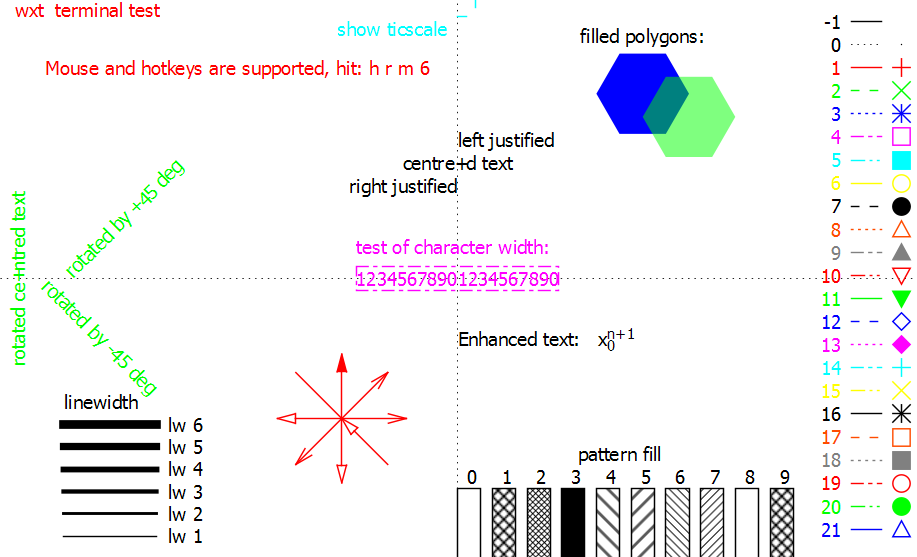
\includegraphics[width=1.0\textwidth]{02_beispiel_kapitel/Testseite.PNG}
    \caption{Gnuplot-Testseite mit Information zu Linientypen, Farben, etc.}
    \label{fig:Testseite}
  \end{center}
 \end{figure}


\section{Literatur-Bibliothek verwalten}
Falls ein externes Literaturverwaltungsprogramm wie z.B. Zotero verwendet wird,
kann ein .bib-Datei ausgegeben werden. Diese Datei kann dann die Datei literatur.bib
ersetzen. Manuell kann natürlich die Datei literatur.bib durch weitere Einträge
ergänzt werden. Je nach Art der Literatur wird die Quelle mit @book, @phdthesis,
@article, @incollection\ldots angegeben.
\begin{verbatim}
@INCOLLECTION{ramm_vs_foerster_wall:2008,
  author = {Ramm, E. and  {von Scheven}, M. and  Förster, Ch. and  Wall, W.A.},
  title = {Interaction of incompressible flows and thin-walled structures},
  booktitle = {ECCOMAS Multidisciplinary Jubilee Symposium. New Computational
    Challenges in Materials, Structures and Fluids},
  publisher = {Computational Methods in Applied Sciences, 14, Springer-Verlag,
  Berlin, Heidelberg},
  year = {2008},
  pages = {219--233},
  otherinfo = {}
\end{verbatim}
Am Ende treten im Literaturverzeichnis nur die Quellen auf, die im Text
zitiert wurden. Je nachdem ob die Quelle im Satzfluss verwendet
(Laut \cite{bischoff:1999} kann eine Schale\ldots) oder als Ergänzung verwendet
wird (Die Interaktion von inkompressiblen Flüssen und dünnwandigen Sturkturen
kann berücksichtigt werden \citep{ramm_vs_foerster_wall:2008})
werden Klammern um die Quelle gesetzt oder nicht. Dazu werden zwei verschiedene
Befehle verwendet: im ersten Fall wäre dies
\verb+\cite{bischoff:1999}+ im zweiten
\verb+\citep{ramm_vs_foerster_wall:2008}+.

Die Verzeichnisse (Literaturverzeichnis und Inhaltsverzeichnis) werden erst beim
zweimaligen Übersetzen aktualisiert.






    %&latex {


%%%%%%%%%%%%%%%%%%%%%%%%%%%%%%%%%%%%%%%
%
%   Z U S A M M E N F A S S U N G
%
%%%%%%%%%%%%%%%%%%%%%%%%%%%%%%%%%%%%%%%
\chapter{Zusammenfassung und Ausblick}
\label{zusammen}


Hier sollte die Arbeit zusammengefasst werden. Außerdem wäre es gut, einen
Ausblick zu geben, wie die Arbeit fortgeführt werden könnte
oder was noch verbessert werden müsst. 








    %%%%%%%%%%%%%%%%%%%%%%%%%%%%%%%%%%%%%%%%%%%%%%%%%
    %
    % NACHSPANN:
    % - Literaturverzeichnis
    %
    %%%%%%%%%%%%%%%%%%%%%%%%%%%%%%%%%%%%%%%%%%%%%%%%%
    \nachspann
    \begin{spacing}{1.1}
        \bibliographystyle{\bst}
        \bibliography{literatur}
    \end{spacing}



    %%%%%%%%%%%%%%%%%%%%%%%%%%%%%%%%%%%%%%%%%%%%%%%%%
    %
    % Anhang (optional)
    %
    %%%%%%%%%%%%%%%%%%%%%%%%%%%%%%%%%%%%%%%%%%%%%%%%%
    \begin{appendix}
        \begin{spacing}{1.1}
            \chapter{Messdaten}
            \label{ch:messdaten}

        \end{spacing}
    \end{appendix}


\end{document}

